\section{Física}
\subsection{Vectores}
\begin{enumerate}
	\item Para los vectores:
	\begin{align*}
		\vb{A} &= \vx + \vy - 2\vz \\
		\vb{B} &= 3\vx - 2\vy - \vz \\
		\vb{C} &= \vy - 5\vz
	\end{align*}
Calcule:
	\begin{enumerate}[I)]
		\item $\vb{A} + \vb{B}$
		\item $\vb{B} - \vb{C}$
		\item $\vb{A} - \vb{B} - \vb{C}$
		\item $\vb{A} \cdot \vb{B}$
		\item Encuentre el ángulo entre $\vb{A}$ y $\vb{B}$. 
	\end{enumerate}
	\item Para un vector con magnitud $10$ y ángulo respecto al eje $y$ de $\flatfrac{\pi}{4}$rad, encuentre las componentes de dicho vector y escribalas en las dos notaciones aprendidas.
	\item Para el vector $(-8,-6)$ encuentre el ángulo respecto el eje $+x$ y la magnitud de dicho vector.
	\item Utilize el método gráfico para sumar los siguientes vectores (utilize hojas cuadriculadas para facilitar el trabajo): $(3,4)$ y $(6,2)$.
\end{enumerate}

\subsection{Cinemática}
\subsubsection{MRU}
	\begin{enumerate}
		\item Tres niños en un estacionamiento lanzan un cohete que se eleva en el aire por un arco de $380 m$ de longitud en $40 s$.
Determine la rapidez promedio.
		\item Un automóvil viaja a razón de $25km/h$ durante $4min$, después a $50km/h$ durante $8min$, y por último a $20km/h$ durante $2min$. Encuentre la distancia total cubierta y la rapidez promedio del viaje.
		\item Desde el centro de una ciudad, un vehículo viaja hacia el este durante $80.0 km$ y luego da vuelta al sur durante otros
$192 km$, hasta que se le acaba la gasolina. Determinar el desplazamiento del automóvil detenido desde el centro de la
ciudad.
		\item Una embarcación viaja justo hacia el este a $10 km / h$. ¿Cuál debe ser la rapidez de una segunda embarcación que se
dirige $30^o$ al noreste si siempre está directamente al norte de la primera embarcación?
	\end{enumerate}
\subsubsection{MRUV}
	\begin{enumerate}
		\item Un automóvil viaja a $20.0 m / s$ cuando el conductor pisa los frenos y se detiene en una línea recta en $4.2 s$.
¿Cuál es la magnitud de su aceleración media?
		\item Se lanza una pelota verticalmente hacia arriba en la Luna y regresa a su punto de partida en $4.0 s$. La
aceleración debida a la gravedad en ese lugar es de $1.60 m / s^2$ . Encuentre la rapidez inicial.
		\item Desde un globo que está a $300 m$ sobre el suelo y se eleva a $13 m / s$, se deja caer una bolsa de lastre.
Para la bolsa, encuentre: a) la altura máxima que alcanza, b) su posición y velocidad después de $5.0 s$ de
haberse desprendido y c) el tiempo que tarda en bajar y golpear el suelo.
		\item Un tren subterráneo en reposo parte de una estación y acelera a una tasa de $1.60m/s^2$ durante $14.0s$. Viaja con una rapidez constante de $70.0s$ y frena a $3.5m/s^2$ hasta detenerse en la siguiente estación. Calcule la distancia total cubierta.
		\item Un vehículo espacial está descendiendo hacia la Base Lunar $I$, desciende lentamente gracias al retroempuje del motor de descenso. EL motor se apaga cuando el vehículo está a $5.0m$ sobre la superficie y tiene una velocidad descendente de $0.8m/s$. Con el motor apagado, el vehículo está en caída libre. ¿Qué rapidez tiene justno antes de tocar la superficie? La aceleración debida a la gravedad lunar es de $1.6m/s^2$.
		\item El tripulante de un globo areostático, que sube verticalmente con velocidad constante de magnitud $5.0m/s$, suelta un saco de arena cuando el globo está a $40.0m$ sobre el suelo. No hay resistencia del aire. $a)$ Calcule la posición y velocidad del saco a $0.250s$ y $1.00s$ despues de soltarse. $b)$ ¿Cuántos segundos tardará el saco en chocar con el suelo después de soltarse? $c)$ ¿Con que velocidad chocará? $d)$ ¿Qué altura máxima alcanza el saco en relación con el suelo? $e)$ Dibuje cualitativamente las gráficas $v_y - t$ y $y-t$ para el movimiento. Recuerde dejar en claro cual es su sistema de referecia.
		\item El maquinista de un tren de pasajeros que se mueve
a $25.0 m/s$ avista un tren de carga cuyo último vagón está $200 m$ más adelante en la misma vía. El tren de carga se mueve
con una rapidez de $15.0 m/s$ en la misma dirección que el tren de
pasajeros. El maquinista del tren de pasajeros aplica de inmediato los
frenos, causando una aceleración constante de $0.100 m/s^2$, en dirección
opuesta a la de la velocidad del tren, mientras el tren de carga
sigue con rapidez constante. Sea $x = 0$ el punto donde está la parte
frontal del tren de pasajeros cuando el maquinista aplica los frenos.
a) ¿Atestiguarán las vacas de los alrededores una colisión? b) Si es
así, ¿dónde ocurrirá?
	\end{enumerate}
\subsubsection{Movimiento Parabólico}
	\begin{enumerate}
		\item Un mariscal de campo novato lanza un balón con una componente
        de velocidad inicial hacia arriba de $12.0 \velocity$ y una componente
        de velocidad horizontal de $20.0 \velocity$. Ignore la resistencia del aire.
        $a)$ ¿Cuánto tiempo tardará el balón en llegar al punto más alto de la
        trayectoria? $b)$ ¿A qué altura está este punto? $c)$ ¿Cuánto tiempo pasa
        (desde que se lanza) para que el balón vuelva a su nivel original?
        ¿Cómo se compara este tiempo con el calculado en el inciso $a)$?
        $d)$ ¿Qué distancia horizontal viaja el balón en este tiempo? $e)$ Dibuje
        las gráficas $x-t$, $y-t$, $v_x-t$ y $v_y-t$ para el movimiento (dibujelas aproximadas no es necesario que las dibuje exactas).
        \item En una feria, se puede ganar una jirafa de
peluche lanzando una moneda a un platito, el cual está sobre una repisa
más arriba del punto en que la moneda sale de la mano y a una distan-
cia horizontal de $2.1 m$ desde ese punto. Si usted lanza
la moneda con velocidad de $6.4 m/s$, a un ángulo de $60^o$ sobre la horizontal, la moneda caerá en el platito. Ignore la resistencia del aire. a) ¿A qué altura está la repisa sobre el punto donde se lanza la moneda?
b) ¿Qué componente vertical tiene la velocidad de la moneda justo
antes de caer en el platito?
		\begin{figure}[H]
			\centering
			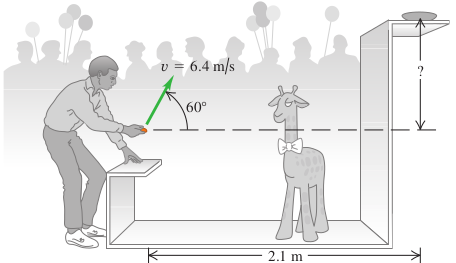
\includegraphics[scale=0.5]{Images/feria.png}
			\caption{Figura del problema $1.2.3.2.$}
			\label{1.2.3.2}
		\end{figure}
		\item Conforme un barco se acerca al muelle a $45.0 cm/s$, es nece-
sario lanzarle la pieza de un equipo importante para que pueda atracar.
El equipo se lanza a $15.0 m/s$ a $60.0^o$ por encima de la horizontal
desde lo alto de una torre en la orilla del agua, a $8.75 m$ por encima de
la cubierta del barco. Para que el equipo caiga enfrente
del barco, ¿a qué distancia $D$ del muelle debería estar el barco cuando
se lance el equipo? Se ignora la resistencia del aire.
		\begin{figure}[H]
			\centering
			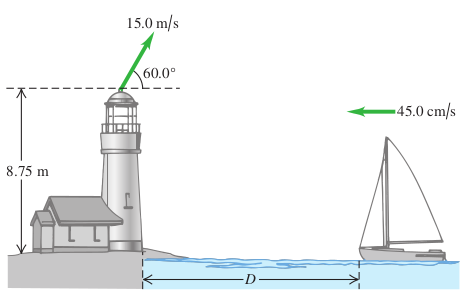
\includegraphics[scale=0.5]{Images/barco.png}
			\caption{Figura del problema $1.2.3.3.$}
			\label{1.2.3.2}
		\end{figure}
	\end{enumerate}

\subsection{Dinámica}
	\begin{enumerate}
		\item Usted entra en un elevador, se para sobre una báscula y oprime
el botón de “subir”. También recuerda que su peso normal es de $625 N$.
Comience a contestar cada una de las siguientes preguntas dibujando
un diagrama de cuerpo libre. a) Si el elevador tiene una aceleración de
$2.50 m/s^2$ , ¿cuánto se lee en la báscula? b) Si usted sostiene desde el
inicio un paquete de $3.85 kg$ con una cuerda vertical ligera, ¿cuál es la
tensión en la cuerda una vez que el elevador comienza a acelerar?
		\item Un anuncio asegura que cierto automóvil puede “dete-
nerse en una moneda de 10 centavos”. ¿Qué fuerza neta sería necesaria
para detener un auto de $850 kg$ que viaja a $45.0 km/h$ en una distancia
igual al diámetro ($1.8 cm$) de una moneda de 10 centavos de dólar?
			\pagebreak
		\item 
\begin{multicols}{2}
Dos cuerdas están unidas a Figura un cable de acero que sostiene una
pesa que cuelga. a) Dibuje un diagrama
de cuerpo libre que muestre todas las
fuerzas que actúan sobre el nudo que
une las dos cuerdas al cable de acero.
Con base en su diagrama de fuerzas,
¿cuál cuerda estará sometida a mayor
tensión? b) Si la tensión máxima que una cuerda resiste sin romperse
es de $5000 N$, determine el valor máximo de la pesa que las cuerdas
pueden sostener sin riesgo. Puede despreciarse el peso de las cuerdas y
del cable de acero.
\columnbreak
\begin{figure}[H]
	\centering
	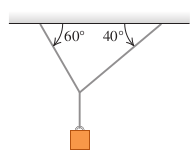
\includegraphics[scale=0.6]{Images/tension.png}
	\caption{Figura del problema $1.3.3.$}
	\label{1.3.2.}
\end{figure}
\end{multicols}
		\item El bloque que se muestra en la figura \ref{tresbloques}a se desliza con una rapidez constante bajo la acción de la fuerza
mostrada. a) ¿Cuán grande es la fuerza de fricción retardadora? b) ¿Cuál es el coefi ciente de fricción cinética
entre el bloque y la superficie?
		\item El bloque que se muestra en la figura \ref{tresbloques}b se desliza hacia abajo con rapidez constante. a) ¿De cuánto es
la fuerza de fricción que se opone a su movimiento? b) ¿Cuál es el coeficiente de fricción de deslizamiento
(cinética) entre el bloque y el plano?
		\item El bloque de la figura \ref{tresbloques}c empieza a deslizarse hacia arriba de la pendiente cuando la fuerza de empuje
mostrada se incrementa a $70 N$. a) ¿Cuál es la fuerza de fricción estática máxima sobre él? b) ¿Cuál es el valor
del coefi ciente de fricción estática?
	\end{enumerate}
		\begin{figure}[H]
			\centering
			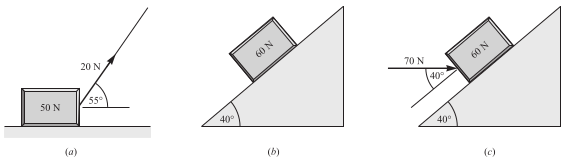
\includegraphics[scale=0.6]{Images/tresbloques.png}
			\caption{Problemas $1.3.4$, $1.3.5$ y $1.3.6$}
			\label{tresbloques}
		\end{figure}


\subsection{Trabajo, Energía y Momentum Lineal}
\begin{enumerate}
	\item Suponga que un objeto se jala con una fuerza de $75 N$ en la dirección de $28^o$ sobre la
horizontal. ¿Cuánto trabajo desarrolla la fuerza al tirar del objeto $8.0 m$?
	\item Como se muestra en la figura siguiente, una cuenta se desliza sobre un alambre. Si la fuerza de fricción es des-
preciable y en el punto A la cuenta tiene una rapidez de $200 cm/s$, a) ¿cuál será su rapidez en el punto B?,
b) ¿cuál en el punto C?
		\begin{figure}[H]
			\centering
			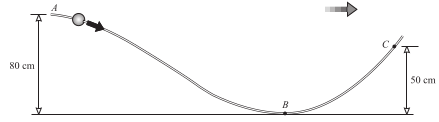
\includegraphics[scale=0.6]{Images/alambre.png}
			\caption{Problema $1.4.2$}
			\label{tresbloques}
		\end{figure}
	\item Justo antes de chocar con el piso, una masa de $2.00 kg$ tiene $400 J$ de EC. Si se desprecia la fricción, ¿de qué
altura se dejó caer dicha masa?
	\item El conductor de un automóvil de $1 200 kg$ observa que la rapidez de su automóvil disminuye de $20 m/s$ a
$15 m/s$ mientras recorre una distancia de $130 m$ sobre suelo nivelado. ¿De qué magnitud es la fuerza que se
opone al movimiento del automóvil?
	\item Una bomba de agua sube el líquido desde un lago hasta un gran tanque colocado $20 m$ arriba del nivel del lago.
¿Cuánto trabajo contra la gravedad efectuará la bomba para transferir $5.0 m^3$ de agua al tanque? Un metro
cúbico de agua tiene una masa de $1 000 kg$.
	\item Por lo general, una pelota de tenis golpeada durante un servicio viaja a alrededor de $51 m/s$. Si la pelota se
encuentra en reposo en medio del aire al ser golpeada y tiene una masa de $0.058 kg$, ¿cuál es el cambio en su
cantidad de movimiento al salir de la raqueta?
	\item Un camión de carga vacío de $15 000 kg$ viaja por una pista plana a $5.00 m/s$. Súbitamente se dejan caer dentro
del camión, directamente desde arriba, $5 000 kg$ de carbón. Inicialmente, la velocidad del carbón en la dirección horizontal es cero con respecto al suelo. Encuentre la rapidez final del camión.	
	\item Dos pelotas idénticas que viajan paralelas al eje $x$ tienen rapideces de $30 cm/s$, en sentidos opuestos. Sufren
una colisión perfectamente elástica fuera de sus centros. Después del choque, una de las pelotas se mueve en
un ángulo de $30^o$ sobre el eje $+x$. Encuentre su rapidez y la velocidad de la otra pelota.
\end{enumerate}

\section{Matemática}
\subsection{Álgebra}
\subsubsection{Ecuaciones}
Resuelva $3$ ejercicios por el método gráfico y el resto por el método analítico.
\begin{enumerate}
	\item $
			\left\{
			\begin{array}{rcl}
				x+2y & = & 7 \\
				5x-y & = & 2
			\end{array}
			\right.
		$
		\item $
			\left\{
			\begin{array}{rcl}
				3x+2y & = & 8 \\
				x-2y & = & 0
			\end{array}
			\right.
		$
		\item $
			\left\{
			\begin{array}{rcl}
				4x+2y & = & 16 \\
				x-5y & = & 70
			\end{array}
			\right.
		$
		\item $
			\left\{
			\begin{array}{rcl}
				2x-6y & = & 10 \\
				-3x+9y & = & -15
			\end{array}
			\right.
		$
		\item $
			\left\{
			\begin{array}{rcl}
				x+y & = & 4 \\
				-x+y & = & 0
			\end{array}
			\right.
		$
		\item $
			\left\{
			\begin{array}{rcl}
				2x-3y & = & 9 \\
				4x+3y & = & 9
			\end{array}
			\right.
		$
\end{enumerate}

\subsubsection{Polinomios}
\begin{enumerate}
	\item Resuelva las siguientes divisiones de polinomios por el método que prefiera, escriba la respuesta de la siguiente forma $P(x) = D(X)\cdot Q(x) + R(x)$, donde $P(x)$ es el polinomio dividendo, $D(x)$ el divisor, $Q(x)$ el cociente y $R(x)$ el residuo.
	\begin{enumerate}[a)]
		\item $P(x) = 3x^2 + 5x - 4$, $D(x) = x + 3$.
		\item $P(x) = x^3 + 4x^2 - 6x + 1$, $D(x) = x - 1$.
		\item $P(x) = x^4 - x^3 + 4x + 2$, $D(x) = x^2 + 3$.
		\item $P(x) = 2x^5 + 4x^4 - 4x^3 - x - 3$, $D(x) = x^2 - 2$.
	\end{enumerate}
	\item Encuentre todos los ceros racionales posibles de los siguientes polinomios y verifique cuales de ellos son ceros.
	\begin{enumerate}[a)]
		\item $P(x) = x^4 - 3x^3 - 6x + 8$.
		\item $P(x) = 12x^5 + 6x^3 - 2x - 8$.
		\item $P(x) = 6x^4 - x^2 + 2x + 12$.
		\item $P(x) = 8x^3 + 10x^2 - x - 3$.
	\end{enumerate}
	\item Encuentre todos los ceros racionales posibles de los siguientes polinomios y verifique cuales de ellos son ceros y escriba el polinomio de forma factorizada. Además, bosqueje la grafica del polinomio utilizando toda la información útil (corte en $y$, multiplicidades y la tendencia inicial y final del polinomio).
	\begin{enumerate}[a)]
		\item $P(x) = x^4 + 6x^3 + 7x^2 - 6x - 8$.
		\item $P(x) = 2x^3 - 10x^3 - 9x^2 + 40 x - 12$.
		\item $P(x) = 20x^3 - 8x^2 - 5x + 2$.
		\item $P(x) = 6x^4 - 7x^3 - 12x^2 + 3x - 4$.
		\item $P(x) = 2x^6 - 3x^5 - 13x^4 + 29x^3 - 27x^2 + 32x - 12$.
		\item $P(x) = x^3 + 3x^2 - 4$.
		\item $P(x) = x^2 + 1$.
		\item $P(x) = x^3 + 3x^2 - x - 3$.
		\item $P(x) = x^4 - 2x^3 - 3x^2 + 8x - 4$.
	\end{enumerate}
\end{enumerate}

\subsection{Trigonometría}
\subsubsection{Triángulos y medición de Ángulos}
\begin{enumerate}
	\item Utilizando los catetos y la hipotenusa dada, encontrar todos los ángulos de su respectivo triangulo rectangulo:
	\begin{enumerate}[a)]
		\item $c_1 =3$, $c_2 =4$ y $h=5$.
		\item $c_1 =6$, $c_2 =6$ y $h=6\sqrt{2}$.
		\item $c_1 =8\sqrt{15}$, $c_2 =14$ y $h=34$.
		\item $c_1 =\sqrt{5}$, $c_2 =2$ y $h=3$.
	\end{enumerate}
	\item Encuentre el valor del lado o ángulo que se solicita.
	\begin{enumerate}[a)]
		\begin{multicols}{2}
			\item 
				\begin{figure}[H]
					\centering
					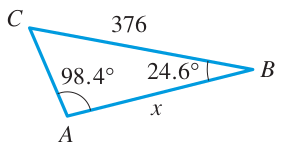
\includegraphics[scale=0.3]{Images/t1.png}
				\end{figure}
			\item 
			\begin{figure}[H]
				\centering
				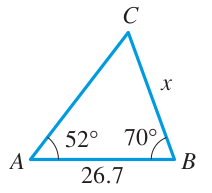
\includegraphics[scale=0.3]{Images/t2.png}
			\end{figure}
			\item 
			\begin{figure}[H]
				\centering
				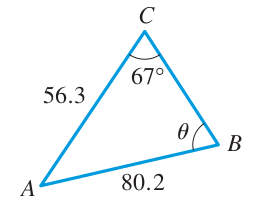
\includegraphics[scale=0.3]{Images/t3.png}
			\end{figure}
			\item 
			\begin{figure}[H]
				\centering
				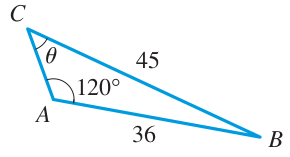
\includegraphics[scale=0.3]{Images/t4.png}
			\end{figure}
			\item 
			\begin{figure}[H]
				\centering
				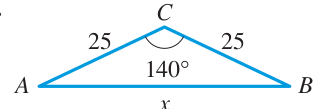
\includegraphics[scale=0.3]{Images/t5.png}
			\end{figure}
			\item 
			\begin{figure}[H]
				\centering
				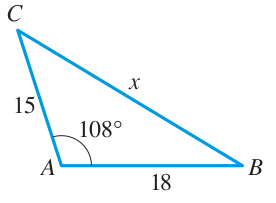
\includegraphics[scale=0.3]{Images/t6.png}
			\end{figure}
			\item 
			\begin{figure}[H]
				\centering
				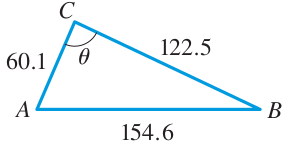
\includegraphics[scale=0.3]{Images/t7.png}
			\end{figure}		
		\end{multicols}
	\end{enumerate}
	\item Para probemas de aplicación, se recomienda el libro de Stewart, capítulo 6.
\end{enumerate}


\subsection{Geometría}
\subsubsection{Áreas Sombreadas}
\begin{enumerate}
	\item Encuentre el valor del área sombreada.
	\begin{enumerate}[a)]
		\begin{multicols}{2}
			\item 
				\begin{figure}[H]
					\centering
					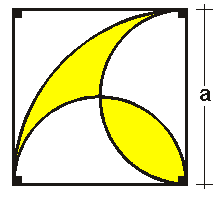
\includegraphics[scale=0.5]{Images/a1.png}
				\end{figure}
			\item 
			\begin{figure}[H]
				\centering
				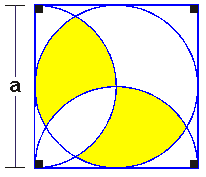
\includegraphics[scale=0.5]{Images/a2.png}
			\end{figure}
			\item 
			\begin{figure}[H]
				\centering
				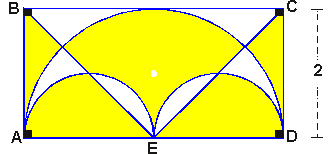
\includegraphics[scale=0.5]{Images/a3.png}
			\end{figure}
			\item Diametro $4$
			\begin{figure}[H]
				\centering
				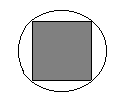
\includegraphics[scale=0.5]{Images/a4.png}
			\end{figure}
			\item Lado $l = 2$
			\begin{figure}[H]
				\centering
				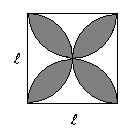
\includegraphics[scale=0.5]{Images/a5.png}
			\end{figure}		
		\end{multicols}
	\end{enumerate}
\end{enumerate}
